% -*- TeX-engine: xetex; eval: (auto-fill-mode 0); eval: (visual-line-mode 1); -*-
% Compile with XeLaTeX

\documentclass[11pt]{article}
%%%%%%%%%%%%%%%%
% Packages
%%%%%%%%%%%%%%%%

\usepackage[top=1cm,bottom=1cm,left=1.5cm,right= 1.5cm]{geometry}
\usepackage[parfill]{parskip}
\usepackage{graphicx, fontspec, xcolor, multicol, enumitem, setspace}
\DeclareGraphicsRule{.tif}{png}{.png}{`convert #1 `dirname #1`/`basename #1 .tif`.png}

%%%%%%%%%%%%%%%%
% Sakai link - update each semester
%%%%%%%%%%%%%%%%

\newcommand{\Sakai}[1]
{\href{https://sakai.duke.edu/portal/site/ef372254-413e-42f6-b414-f8bc91a58fa0/page/98390abf-b461-44cb-a062-aa6864748ab3}{Sakai}}


%%%%%%%%%%%%%%%%
% No page number
%%%%%%%%%%%%%%%%

\pagestyle{empty}

%%%%%%%%%%%%%%%%
% User defined colors
%%%%%%%%%%%%%%%%

% Pantone 2015 Spring colors
% http://iwork3.us/2014/09/16/pantone-2015-spring-fashion-report/
% update each semester or year

\xdefinecolor{custom_blue}{rgb}{0, 0.70, 0.79} % scuba blue
\xdefinecolor{custom_darkBlue}{rgb}{0.11, 0.31, 0.54} % classic blue
\xdefinecolor{custom_orange}{rgb}{0.97, 0.57, 0.34} % tangerine
\xdefinecolor{custom_green}{rgb}{0.49, 0.81, 0.71} % lucite green
\xdefinecolor{custom_red}{rgb}{0.58, 0.32, 0.32} % marsala

\xdefinecolor{custom_lightGray}{rgb}{0.78, 0.80, 0.80} % glacier gray
\xdefinecolor{custom_darkGray}{rgb}{0.54, 0.52, 0.53} % titanium

%%%%%%%%%%%%%%%%
% Color text commands
%%%%%%%%%%%%%%%%

%orange
\newcommand{\orange}[1]{\textit{\textcolor{custom_orange}{#1}}}

% yellow
\newcommand{\yellow}[1]{\textit{\textcolor{yellow}{#1}}}

% blue
\newcommand{\blue}[1]{\textit{\textcolor{blue}{#1}}}

% green
\newcommand{\green}[1]{\textit{\textcolor{custom_green}{#1}}}

% red
\newcommand{\red}[1]{\textit{\textcolor{custom_red}{#1}}}

%%%%%%%%%%%%%%%%
% Coloring titles, links, etc.
%%%%%%%%%%%%%%%%

\usepackage{titlesec}
\titleformat{\section}
{\color{custom_blue}\normalfont\Large\bfseries}
{\color{custom_blue}\thesection}{1em}{}
\titleformat{\subsection}
{\color{custom_blue}\normalfont}
{\color{custom_blue}\thesubsection}{1em}{}

\newcommand{\ttl}[1]{ \textsc{{\LARGE \textbf{{\color{custom_blue} #1} } }}}

\newcommand{\tl}[1]{ \textsc{{\large \textbf{{\color{custom_blue} #1} } }}}

\usepackage[colorlinks=false,pdfborder={0 0 0},urlcolor= custom_orange,colorlinks=true,linkcolor= custom_orange, citecolor= custom_orange,backref=true]{hyperref}

%%%%%%%%%%%%%%%%
% Instructions box
%%%%%%%%%%%%%%%%

\newcommand{\inst}[1]{
\colorbox{custom_blue!20!white!50}{\parbox{\textwidth}{
	\vskip10pt
	\leftskip10pt \rightskip10pt
	#1
	\vskip10pt
}}
\vskip10pt
}

%%%%%%%%%%%
% App Ex number    %
%%%%%%%%%%%

% DON'T FORGET TO UPDATE

\newcommand{\appno}[1]
{5.3}

%%%%%%%%%%%%%%
% Turn on/off solutions       %
%%%%%%%%%%%%%%

% Off
\newcommand{\soln}[1]{}

%% On
%\newcommand{\soln}[1]{
%\textit{\textcolor{custom_darkGray}{#1}}
%}

%%%%%%%%%%%%%%%%
% Document
%%%%%%%%%%%%%%%%

\begin{document}
\fontspec[Ligatures=TeX]{Helvetica Neue Light}

Dr. \c{C}etinkaya-Rundel \hfill Data Analysis and Statistical Inference \\

\ttl{Application exercise \appno{}: \\
Chi-square testing}

\inst{Submit your responses on \Sakai{}, under the appropriate assignment. Only one submission per team is required. One team will be randomly selected and their responses will be discussed.}

\section*{American National Election Survey}

The American National Election Studies (ANES) aims to inform explanations of election outcomes by providing data that support rich hypothesis testing, maximize methodological excellence, measure many variables, and promote comparisons across people, contexts, and time. In this question we will focus on two variables from the 2012 ANES dataset: 
\begin{itemize}
\item region (levels: Northeast, North Central, South, and West), and
\item whether the respondent feels things in this country are generally going in the right direction or things have pretty seriously gotten off on the wrong track.
\end{itemize}
To keep calculations simple we will work with a random sample of 500 respondents from the ANES dataset. The distribution of responses are as follows:

\begin{minipage}[c]{0.5\textwidth}
\begin{center}
\begin{tabular}{rrr|r}
  \hline
 & Right  & Wrong  &  \\ 
 &  Direction &  Track & Total \\ 
  \hline
Northeast & 29 & 54 & 83 \\ 
  North Central & 44 & 77 & 121 \\ 
  South & \textit{\textbf{62}} & 131 & 193 \\ 
  West & 36 & 67 & 103 \\ 
\hline
  Total & 171 & 329 & 500 \\ 
   \hline
\end{tabular}
\end{center}
\end{minipage}
\begin{minipage}[c]{0.5\textwidth}
\begin{center}
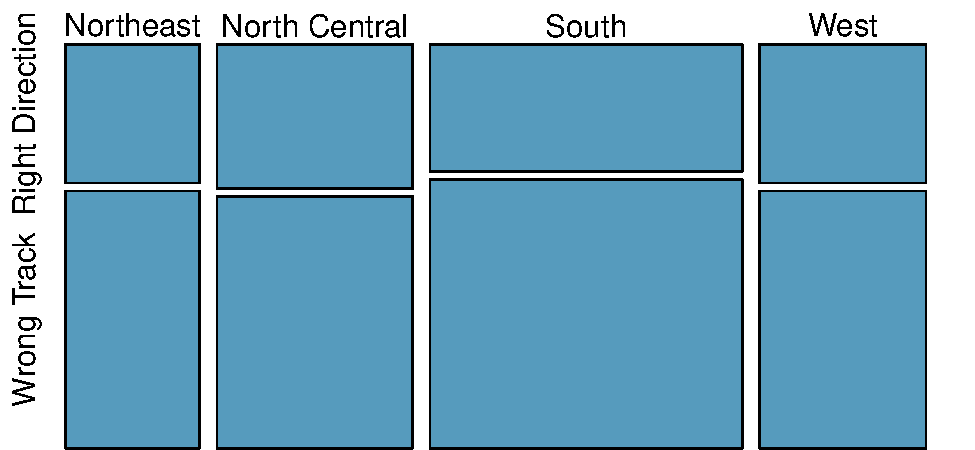
\includegraphics[width=0.95\textwidth]{anes_mosaic}
\end{center}
\end{minipage}

\begin{center}
\textbf{HINT: Read both parts before answering the question.}
\end{center}

\begin{enumerate}

\item \textbf{Part 1:} Region

According to the 2010 Census, 18\% of US residents live in the Northeast, 22\% live in the North Central region, 37\% live in the South, and 23\% live in the North. Evaluate whether the ANES sample is representative of the population distribution of US residents. Make sure to clearly state the hypotheses, check conditions, calculate the appropriate test statistic and the p-value, and make your conclusion in context of the data. \emph{Also} comment on what your conclusion says about whether or not this sample can be considered to be representative.

\soln{$H_0$: The sample distribution of regions follows the census distribution. \\
$H_A$: The sample distribution of regions does not follow the census distribution.
\begin{itemize}
\item Independence:
\begin{itemize}
\item 500 $<$ 10\% of US population
\item Sample is random
\item Each person in the sample is only in one cell
\end{itemize}
\item Sample size: \\
$E_{NE}  500 \times 0.18 = 90$ $\qquad$ $E_{NC}  500 \times 0.22 = 110$ \\
$E_{S}  500 \times 0.37 = 185$ $\qquad$ $E_{W}  500 \times 0.23 = 115$ \\
All expected counts are greater than 5.
\end{itemize}
$\chi^2 = \frac{(83 - 90)^2}{90} + \frac{(121 - 110)^2}{110} + \frac{(193 - 185)^2}{185} + \frac{(103 - 115)^2}{115} \approx 3.24$ \\
$df = 4 - 1 = 3$ \\
$p-value > 0.3$ \\
p-value is large so we fail to reject $H_0$, \\
the data do not provide convincing evidence that the sample distribution of regions does not follow the census distribution. \\
The sample is likely representative since the distribution of sampled individual matches the distribution regional population distribution.
}

\item \textbf{Part 2:} Region and direction
\begin{enumerate}

\item In evaluating the relationship between region and feeling about the direction things are going in the country, what is the response variable and what is the explanatory variable?

\soln{response - direction, explanatory - region}

\item What are the hypotheses for evaluating this relationship?

\soln{$H_0:$ Region and opinion on direction are independent. \\
$H_A:$ Region and opinion on direction are dependent. \\
}

\item If in fact the null hypothesis is true, how many Southerners would we expect to respond that they feel things in this country are generally going in the right direction?

\soln{$E = \frac{193 \times 171}{500} = 66.006$}

\item What is the contribution of this cell (South \& Right direction) to the test statistic?

\soln{$\frac{(62 - 66.006)^2}{66.006} = 0.24313$}

\item Speculate on whether you would expect to reject or not reject the null hypothesis based on the mosaic plot shown above. Explain your reasoning in at most two sentences.

\soln{No, \\
P(right direction $|$ each level of the region variable) is roughly equal, chances are we won't reject $H_0$.}

\end{enumerate}

\end{enumerate}

\end{document}